
\section{System Co-Design: Smart SSD for Web Search Engine}\label{sec:design}
In this section, we discuss the query offloading in web search engine to Smart SSD.
We first explore the design space in Section~\ref{sec:designSpace} to determine what query processing logic could be cost-effectively offloaded,
then show the design architecture of search engine and Smart SSD in Section~\ref{sec:sysArch}.

\subsection{Design Space}\label{sec:designSpace}

The overall research question of the design: \emph{which query processing logic should be executed inside SSD?} We need to understand the advantages and disadvantages of Smart SSD (summarized in Table~\ref{tab:SmartSSDProCon}).

\textbf{Advantages of Smart SSD}. I/O operation in Smart SSD is very fast, because (1) high internal bandwidth, e.g., 5-10$\times$ faster than the host I/O interface~\cite{Do2013QPS,De2013}. The gap is predicated to increase in the future. (2) low I/O latency, because a regular I/O operation needs to go through the conventional thick OS stack, e.g., file system, interrupt, context switch between kernel space and user space, which is collectively called OS software overhead. The software overhead is negligible on hard disks (as I/O is very slow). However, it takes a considerable fraction of time on fast SSDs~\cite{Caulfield2010}\footnote{Some work in computer architecture area propose to bypass OS to better utilize fast SSDs~\cite{Caulfield2010}.}. Thus, it is very suitable to execute \emph{I/O-intensive} operations inside SSD to leverage the high internal bandwidth and low latency.

\textbf{Disadvantages of Smart SSD}. Currently, our Smart SSD prototype suffers from two aspects. (1) Smart SSD embraces low-frequency processors (typically ARM series) to save energy. Thus, processing capability is several times lower compared to host CPUs (e.g., Intel processor)~\cite{Do2013QPS,De2013}; (2) Smart SSD also has a DRAM inside (called device DRAM), access to device DRAM is slower than to host DRAM. Because there is no instruction- and data-cache inside the embedded processor, and also device memory channels are not shared meaning that only one channel is active at one time. Thus, it is not suitable to execute \emph{CPU-intensive} and \emph{memory-intensive} operations inside SSD.

\begin{table}[htbp]
\centering
\begin{tabular}{l|l}\hline\hline
\textbf{Pros}    & \textbf{Cons}\\\hline
P1. High internal bandwidth & C1. CPU is slow \\\hline
P2. Low I/O latency & C2. DRAM access is slow\\\hline\hline
\end{tabular}
\caption{Pros and cons of Smart SSD}\label{tab:SmartSSDProCon}
\end{table}

However, on SSD-based web search engines, I/O is still the bottleneck. Based on our measurement, around 85\% of the time is spent on loading inverted lists from SSD, where Smart SSD shines.

Understanding this, we set to consider what query processing steps, i.e., step X1 -- X5 in Figure~\ref{fig:searchEngineArch}, could be cost-effectively executed inside SSD. We do a rough analysis first, and evaluate them thoroughly in the experiments.

\textbf{Step X1: parse query}. Parsing a query involves a number of CPU-intensive steps, e.g., tokenization, stemming and lemmatization~\cite{M08}. Thus, it is not cost-effectively to be offloaded to SSD.

\textbf{Step X2: get metadata}. The metadata is a key-value pair. The key is a term $t$, the value is the basic information about the on-disk inverted list $\ell$ of $t$, typically offset, length (in bytes), document frequency. The metadata can be obtained from a dictionary file, which is small enough to fit into host memory. Even if not, it takes very few (usually 1 $\sim$ 2) I/O operations if a Btree-like data structure is built for the dictionary table~\cite{M08}. Thus, we do not offload this step.

\textbf{Step X3: get inverted lists}. Each inverted list $\ell$ contains a list of documents that contain the same term $t$.
Typically, all the inverted lists (i.e., of all terms) are too large enough to fit into host memory~\cite{BaezaYates07ICDE,Zhang2008,Risvik2013}, thus, we take a pessimistic way to assume that the inverted lists are stored on SSD.
Reading inverted lists from disk to host memory requires many I/Os, taking around 85\% of the time based on our measurements. Thus, we offload this step to SSD to take the advantage of high internal bandwidth and low latency (see Table~\ref{tab:SmartSSDProCon}).

\textbf{Step X4: execute list operations}. The goal of loading inverted lists to host DRAM is for executing list operations, e.g., intersection. Thus, step X4 and X3 should be paired to be offloaded. Then, the question is to determine what operation(s) could be benefit from Smart SSD. The basic operators include: list \textsf{intersection}, \textsf{union} and \textsf{difference}~\cite{M08}, which are frequently used in many commercial search engines (e.g., Google advanced search\footnote{\url{http://www.google.com/advanced_search}}). We investigate each operation in the following, a simple principle is the output should be much smaller than the input; otherwise, could not save any data movement. Let $A$ and $B$ be two inverted lists (assume $A$ is shorter than $B$ to capture the real case of skewed lists).
\begin{itemize}%[noitemsep, topsep=2pt]
  \item For the \textsf{intersection}, the intersection result is usually much smaller compared to each inverted list, i.e., $|A\cap B| \ll |A| + |B|$. E.g., in Bing search, for 76\% of the queries, the intersection result size is two orders of magnitude smaller than the shortest inverted list involved~\cite{Ding2011}. Similar results are observed in our real datasets. Thus executing intersection inside SSD may be a cost-effective choice, as it can save a lot of host I/O interface bandwidth.

  \item For the \textsf{union}, the union result size can be similar to the total size of the inverted lists. This is because, $|A\cup B| = |A| + |B| - |A\cap B|$, while typically, $|A\cap B| \ll |A| + |B|$, then $|A\cup B| \approx |A| + |B|$. Unless $|A\cap B|$ is similar to $|A| + |B|$. An extreme case is $A = B$, then $|A\cup B| = |A| = |B|$, meaning that, we can save 50\% of data transfer. However, in general, it is not cost-effectively to offload \textsf{union} to Smart SSD.

  \item For the \textsf{difference}, it is to find all the documents in one list but not in the other list. As the operation is ordering-sensitive, we consider two cases: $(A - B)$ and $(B - A)$. For the former case, $|A - B| = |A| - |A\cap B| < |A| \ll |A| + |B|$, i.e., sending the results of $(A - B)$ saves a lot of data transfer. However, the other case may not save much data transfer because $|B - A| = |B| - |A\cap B| \approx |B| \approx |B| + |A|$. In summary, we still consider the \textsf{difference} as a possible operation for query offloading.
\end{itemize}

\textbf{Step X5: similarity computation and ranking}. After the list operation (e.g., intersection) is done, we get a list of qualified documents. While users are interested in the top most relevant documents. Thus, we need to apply a ranking mode (e.g., the standard Okapi BM25 model~\cite{Robertson1994}) to compute the similarity between the query $q$ and every qualified document $d$; then rank the results to return top-$k$ most relevant ones. It is CPU-intensive, following the analysis, it may not be cost-effective to be offloaded. However, it is beneficial when the result size is too big. After step X5, only top-$k$ (e.g., 3) results should be returned, which saves a lot of I/Os. Thus it is a tradeoff. From the design aspect, we consider two options: (1) do not offload step X5, this case, step X5 is done at the host side; (2) offload this step, in this case, step X5 is done at the device side and only top-$k$ results are returned to users.

\begin{table}[htbp]
\centering
\begin{tabular}{l|c|c}\hline\hline
&Non-Ranked & Ranked \\\hline
\textsf{Intersection} & \ding{51} & \ding{51} \\\hline
\textsf{Union} &\ding{55}  & \ding{51}\\\hline
\textsf{Difference} & \ding{51}& \ding{51}\\\hline\hline
\end{tabular}
\caption{Design space}\label{tab:designSpace}
\end{table}
In a summary, we consider offloading the five query operations that could be potentially benefit from Smart SSD: \textsf{intersection}, \textsf{ranked intersection}, \textsf{ranked union}, \textsf{difference}, and \textsf{ranked difference}, see Table~\ref{tab:designSpace}. The offloading of non-ranked operations means that step X3 and X4 will be executed inside device while step X5 is executed at the host side. The offloading of ranked operations means that step X3, X4 and X5 will be executed inside the device. In either case, step X1 and X2 runs at the host side.


\subsection{System Architecture}\label{sec:sysArch}

\begin{figure}[htbp]
  \centering
  \begin{tabular}{ccc}
 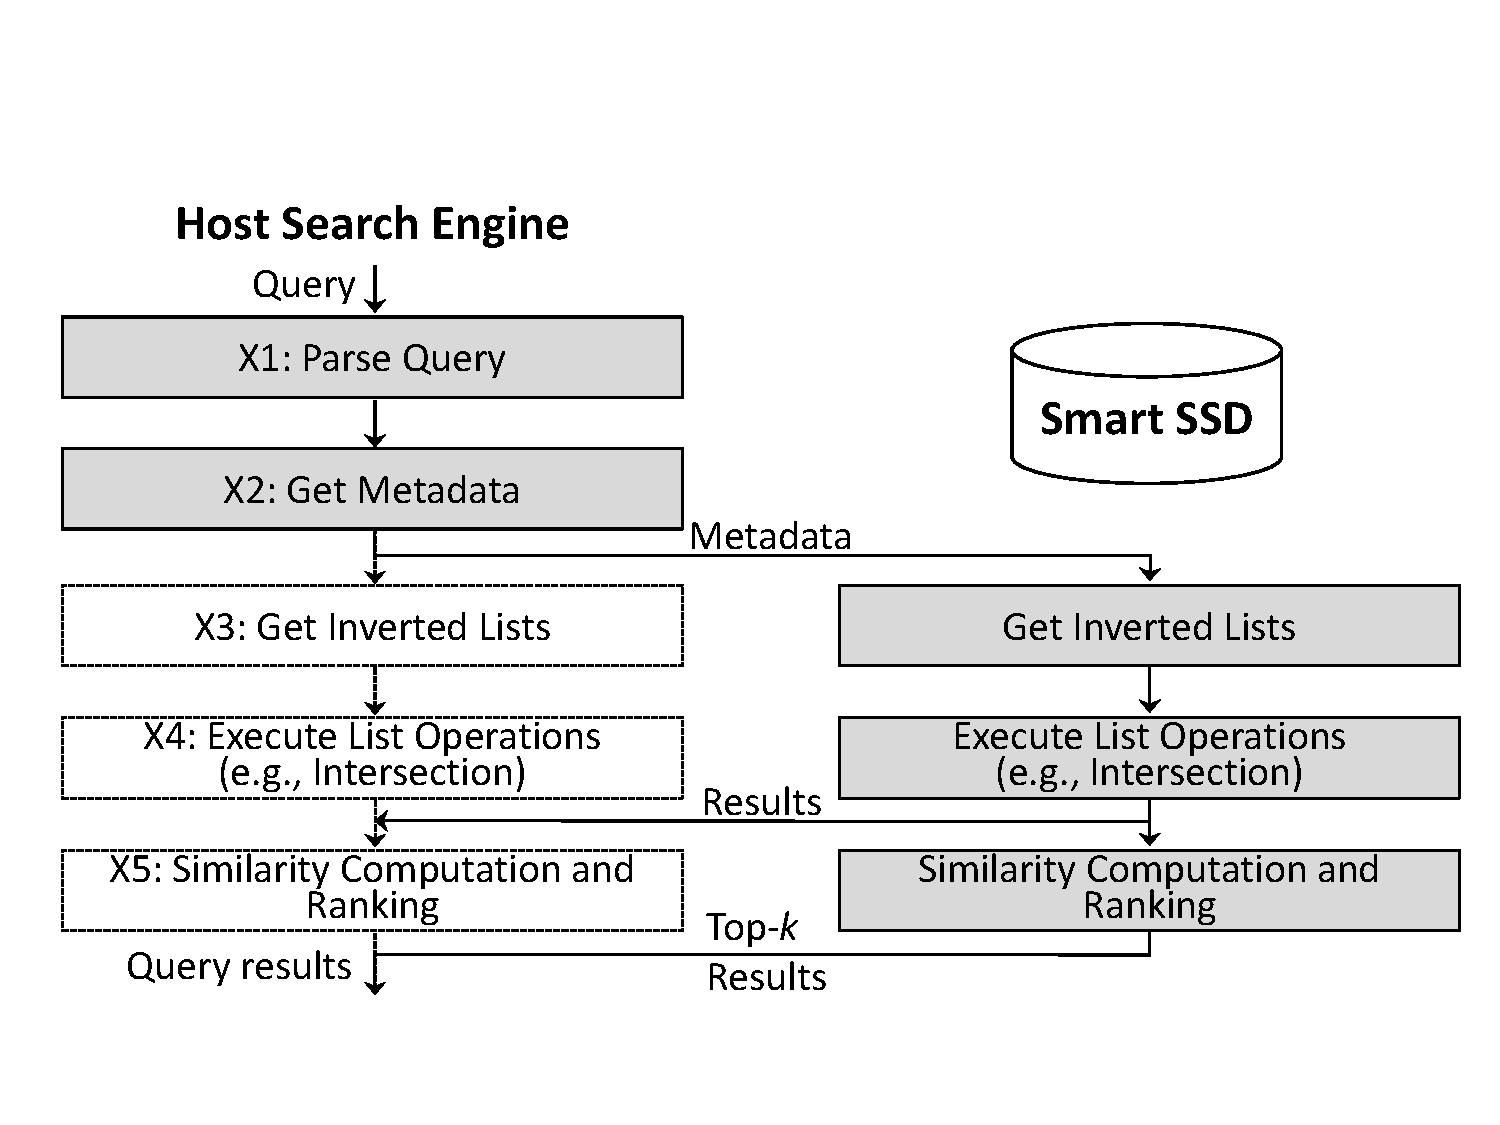
\includegraphics[width=1.0\columnwidth]{figures/SmartSSDLucene.pdf}
\end{tabular}
  \caption{Co-design of web search engine and Smart SSD}
  \label{fig:SmartSSDLucene}
 \end{figure}

Figure~\ref{fig:SmartSSDLucene} shows the design architecture of search engine and SSD, with the query processing logics offloaded.
We integrated Smart SSD with Lucene (an open source search engine) following this architecture. Thus, Lucene can directly interact with Smart SSD.

It works as follows. Assume the intersection operation is offloaded. Upon receiving a query from the host web search engine (e.g., Lucene), it parses the query and get the metadata from host machine (i.e., step X1 and X2 in Figure~\ref{fig:searchEngineArch}). Then, send the metadata to Smart SSD via OPEN API.
In the open function running at Smart SSD, it starts to load the inverted lists to device DRAM. After all the lists are loaded, then execute the list intersection. When the intersection is finished, put the results to the output buffer. The host machine can poll the status of Smart SSD in a heart-beat manner via GET API. We set to  polling interval to be 1ms. When the host side receives the intersection results, it will execute step X5 to finish the query, and return the top ranked results to end users. However, if the ranked operation is offloaded, host machine can directly return results to users upon receiving results from Smart SSD.
